\documentclass[paper.tex]{subfiles}

\begin{document}

\section{Introduction and background}

%once we're finished go back and say exactly how this ended up differing from a knotty ode

This report is heavily based on Robert Ghrist's and Robert Holmes' \emph{An ODE whose solutions contain all knots and links}~\cite{knottyode}.
 In that manuscript, Ghrist gives an excellent high-level exposition of a proof that an ODE containing
all knots and links as periodic orbits exists, building heavily off of his existing work in this area. His manuscript is chock full of interesting side notes; the connection between knot theory and dynamical systems is so rich
that it's difficult to not get distracted by the

Rather than pointlessly recapitulate what Ghrist has already stated so elegantly, we seek to give a more compact and (mostly) self-contained exposition of the beautiful proof that the required ODE exists. The reader is encouraged to
refer to Ghrist's review papers \cite{knottyode}\cite{chaoticknots}to see many many interesting footnotes and connections that will not make it into this work.

We will inevitably be unable to resist the temptation to discuss at least a few interesting connections and questions. The last section of this manuscript is reserved for discussion of those distractions that most fascinate the
authors during the writing.

As briefly stated above, our ultimate goal is to prove the existence of a universal ODE, an ODE whose periodic solutions contain all knots and links.


\subsection{Templates}

The story begins with \emph{templates}, a beautiful and very powerful construction. It would be very difficult to prove the existence of a universal ODE working directly with ODEs, so following one of the main mantras
of mathematics, we collapse out things that are the `same' and obtain a new object. In this case, we collapse out along the stable direction of a given ODE, identifying all orbits which share the same asymptotic future.
This transforms a flow on a three-dimensional manifold into a flow to a semiflow (a one directional flow) on a branched two-dimensional manifold.

We do not discuss the intricacies of this construction, for details, see~\cite{bw1983b}.


\begin{definition}[Template]
  A \emph{template} is a compact branched two-manifold fitted with a smooth expansive semiflow and built from a finite number of \emph{joining} and \emph{splitting} charts, as in Figure~\ref{fig:joinsplit}~\cite{knottyode}.\label{def:template}
\end{definition}


\begin{figure}[h]
  \centering
  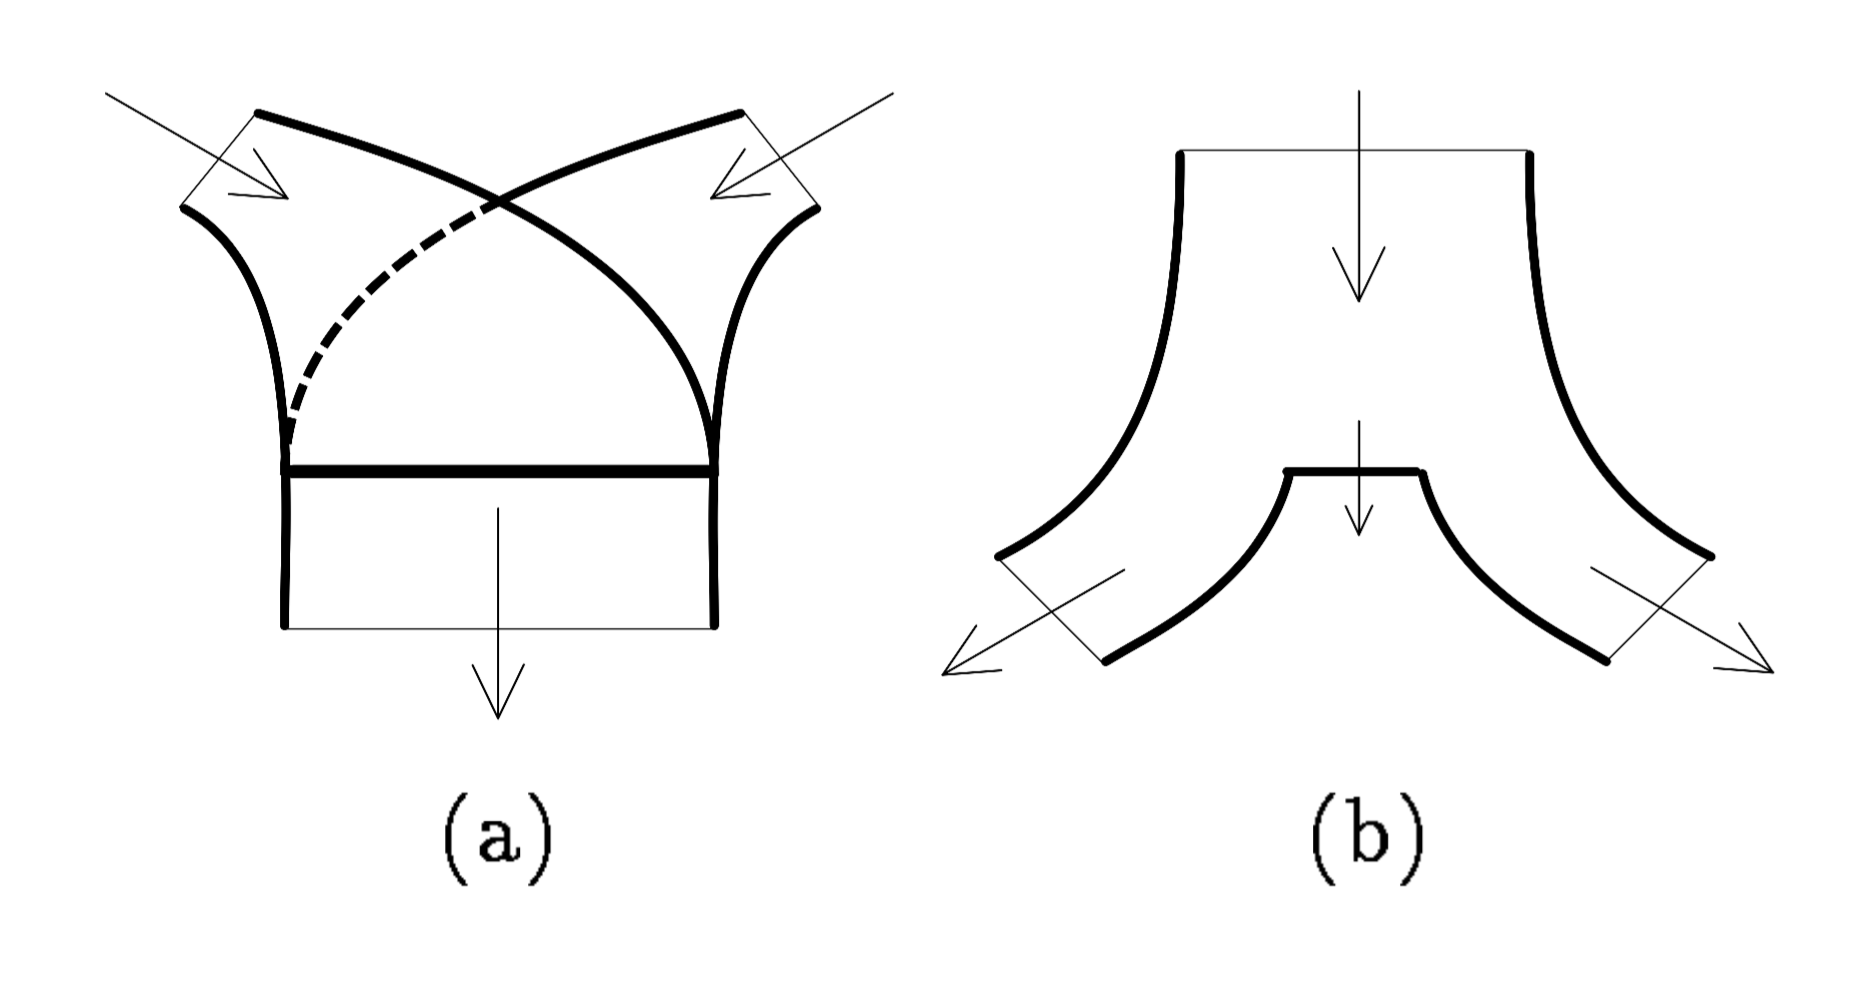
\includegraphics[width=0.5\textwidth]{joining_splitting.png}
  \caption[what goes here]{(a) joining and (b) splitting charts, reproduced from~\cite{knottyode}\protect\footnotemark}\label{fig:joinsplit}
\end{figure}

% how to get this to display?
\footnotetext{Regrettably, without permission}

\begin{figure}[h]
  \centering
  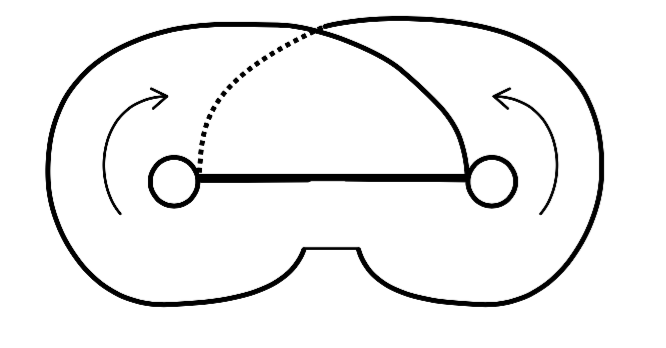
\includegraphics[width=0.5\textwidth]{lorenz.png}
  \caption{The Lorenz template, reproduced from~\cite{knottyode}}\label{fig:lorenz}
\end{figure}

Figure~\ref{fig:lorenz} shows the template for the familiar Lorenz system, the canonical chaotic system, described in equation~\ref{eq:lorenz}. The simplicity of the Lorenz template is a testament to the elegance of
templates - the Lorenz template exactly captures the repeated expanding and folding over of orbits that is the signature of chaos. For certain parameter values, periodic solutions to these equations form a link of infinitely
many components, although we will see later that the Lorenz system is not universal.

\begin{align}
  \label{eq:lorenz}
  \dot{x} &= \sigma(y - x ) \\
  \dot{y} &= \beta x - y - x z \\
  \dot{z} &= - \beta z + x y
\end{align}

The primary formal advantage of working with templates, is that they allow the use of \emph{symbolic dynamics}. We can identify periodic orbits on a template $\tau$ with the sequence of strips crossed.

\begin{definition}
  Following~\cite{knottyode}, given a template $\tau$, we define
  \begin{itemize}
    \item Branch lines  $\set{l_j : j = 1, \cdots M}$, the one-dimensional lines strips are connected along
    \item Strips $\set{x_i : i = 1, \cdots N \geq 2 M}$, the two-dimensional regions connecting branch lines
    \item Itinerary $(x_{s_1}x_{s_2}x_{s_3} \dots)$, a sequence of strips crossed by an orbit on $\tau$
    \item Itinerary space $\Sigma_\tau = \set{a_0 a_1 a_2 \cdots} \subset \set{x_1, x_2, \ldots, x_N}^{\Z^+}$, the set of all possible itineraries on $\tau$
    \item Transition matrix

      \begin{equation}
        A_\tau(i,j) = \left\{ \
        \begin{smallmatrix}
          0 \text{ if } \not\exists \text{ a strip from } x_i \text{ to } x_j \\
          1 \text{ if } \exists \text{ a strip from } x_i \text{ to } x_j
        \end{smallmatrix}
        \right.
      \end{equation}
  \end{itemize}
\end{definition}

It's interesting to note that powers of $A_\tau$ capture allowable trajectories, or more precisely the $(i,j)$th element of the $k$th power of $A_\tau$ will be $1$ iff there is an orbit of $\tau$ of length $k$.
So in principle we have succeeded in reducing questions about the periodic orbits of a flow to questions about powers of a single matrix. Of course, in practice it will be very difficult to compute $A$ from an arbitrary
dynamical system.

See the Figure~\ref{fig:universal} for an example of a template with labeled strips.

Ghrist confirms that the set of admissible sequences on $\sigma_\tau$ corresponds exactly with the set of periodic orbits on $\tau$, as desired.


\subsection{Ordering orbits on templates}

It's possible, and will prove useful, to put an order on orbits on $\tau$. This is accomplished by choosing an ordering on strips emanating from the same branch line and using the induced lexicographic ordering to
order orbits.

This is best illustrated with an example borrowed from~\cite{knottyode}. Let $\V$ be the template illustrated in Figure~\ref{fig:universal}, outfitted with a Markov partition of strips $\set{x_1, x_2, x_3, x_4}$.
Choose an ordering $\vartriangleright$ on the branch lines:

\begin{align}
  l_1 &: x_1 \vartriangleright x_2 \\
  l_2 &: x_3 \vartriangleright x_4
\end{align}

Then a lexicographic ordering on $\sigma_\V$ gives an ordering of orbits. For example, $x_1^2 x_3 x_4 \cdots \vartriangleright x_1 x_2 x_3 x_4 \vartriangleright x_1 x_2 x_4 \cdots$.

Although we have skirted over the details of this ordering here, rest assured that it is well-defined for all templates as confirmed in~\cite{Holmes1989}\cite{Holmes1985}\cite{knottyode}


\subsection{Template renormalization}

Our main tool in proving the existence of a universal template (and by extension a universal ODE) will be \emph{template renormalization}. The following definition are due to~\cite{knottyode}.


% yitz mentioned we need to use a different definition?

% no this sounds fine to me -yitz


\begin{definition}[Subtemplate]
  A \emph{subtemplate} $S \subset \tau$ of a template $\tau$ is a topological subset of $\tau$ which, with the restriction of the semiflow of $\tau$, satisfies the definition of a template (Definition~\ref{def:template})
\end{definition}


\begin{definition}[Template renormalization]
  A  \emph{template renormalization} of a template $\tau$ is a map $\bm{R} : \tau \to \tau$ taking orbits to orbits which is a diffeomorphism onto its image.
  The image of a template renormalization is by definition a subtemplate.
\end{definition}

See Figure~\ref{fig:lorenz_subtemplate} for a helpful illustration of how a renormalization might be constructed.

Note that if a template $\tau$ admits a renormalization, then the image of that renormalization (being diffeormophic to the original template) can again be renormalized, giving an increasingly complicated sequenced of embedded
subtemplates each diffeormorphic to the original! This is the essential property that makes renormalizations such a powerful tool in proving the existence of a universal ODE, a bit later
we will see exactly how its usefulness is manifest.

\begin{figure}[h]
  \centering
  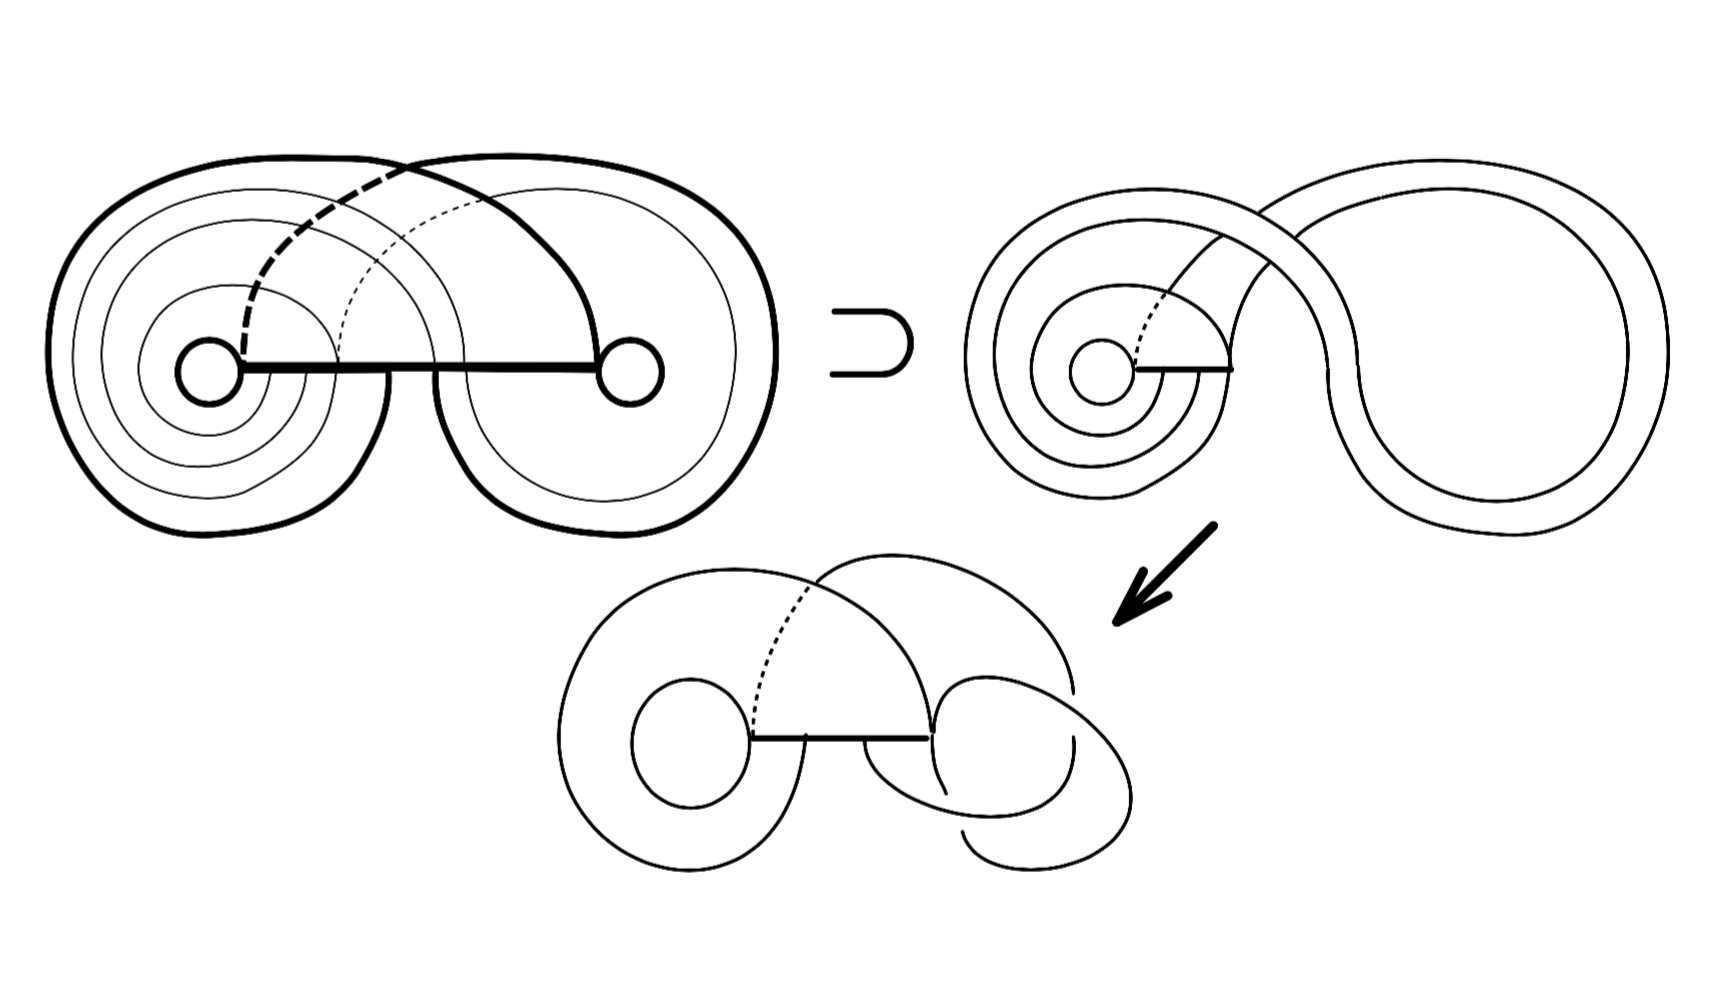
\includegraphics[width=\textwidth]{lorenz_subtemplate.png}
  \caption{A subtemplate of the Lorenz subtemplate $\L$. When it is cut along the boundary and removed from $\L$, it forms a template diffeomorphic to the original one! Figure reproduced from~\cite{knottyode}}\label{fig:lorenz_subtemplate}
\end{figure}

A \emph{very} useful lemma proved in~\cite{knottyode} follows


\begin{lemma}[Ghrist \& Holmes 1993]
  A template renormalization $\bm{R}: \tau \to \tau$ induces a map $\bm{R}: \sigma_\tau \to \sigma_\tau$ whose action is to inflate each element of the Markov partition of strips $\set{x_i : i = 1\cdots N}$ to a finite
  admissible word $\set{\bm{w_i} = w_1 w_2 \cdots w_{n(i)} : i = 1 \cdots N, w_i \in \set{x_i}}$
\end{lemma}

For example the renormalization $\bm{L} : \L \to \L$ shown in Figure~\ref{fig:lorenz_subtemplate} has the following action on the set of strips:

\begin{equation}
  \bm{L} : \L \to \L \left\{ \begin{matrix} & x_1 \mapsto x_1 \\ & x_2 \mapsto x_1 x_2 \end{matrix}\right.
\end{equation}

Renormalizations take knots to knots but will typically change the knot type. We identify a special class of renormalizations that preserve knot type, as these are the renormalizations that we're really after.


\begin{definition}{Isotopic renormalization}
  An \emph{isotopic renormalization} of an embedded template $\tau$ is a template renormalization $\bm{R}$ such that $\bm{R}(\tau)$ is isotopic to $\tau$
\end{definition}

\end{document}
